\newpage
\section{Evasiveness}
Combinatorial Game

Two players: Alice and Bob, graph $G(V,E)$, $|V|=n$.

\begin{figure}[H]
    \centering
    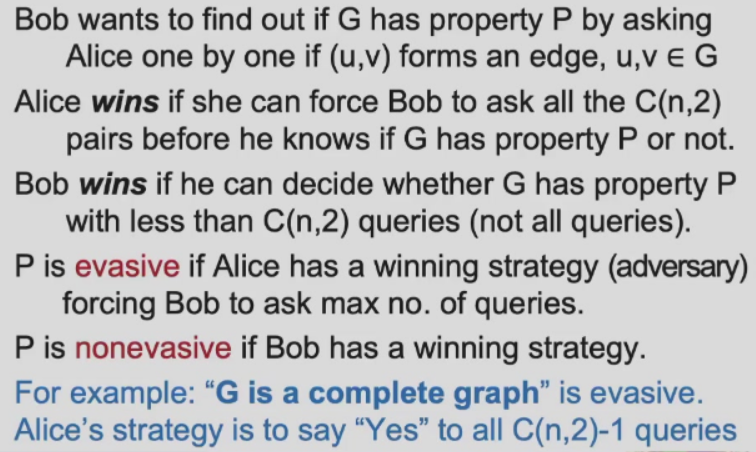
\includegraphics[width=0.309\textwidth]{pic/DAA5/Combinatorial Game}
    \caption{Combinatorial Game}
\end{figure}

\subsection{Evasive Property}
\begin{definition}
    A property is called \textbf{evasive} if determining whether a given graph has this property sometimes requires all possible queries, i.e., $C(n,2)$ queries.
\end{definition}



\begin{itemize}
    \item Empty
    \begin{figure}[H]
        \centering
        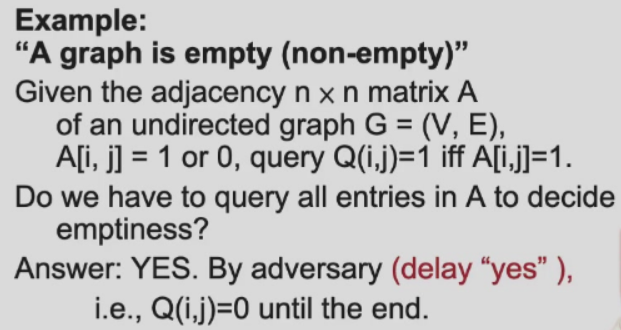
\includegraphics[width=0.309\textwidth]{pic/DAA5/Evasive Property exp}
        \caption{Empty}
    \end{figure}
    \item Number of Edges
    \begin{figure}[H]
        \centering
        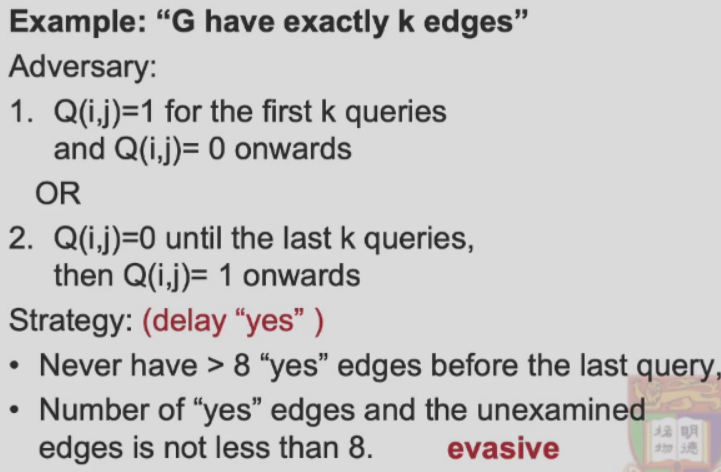
\includegraphics[width=0.309\textwidth]{pic/DAA5/Number of Edges}
        \caption{Number of Edges}
    \end{figure}
    
    \item Graph Connectivity
    \begin{figure}[H]
        \centering
        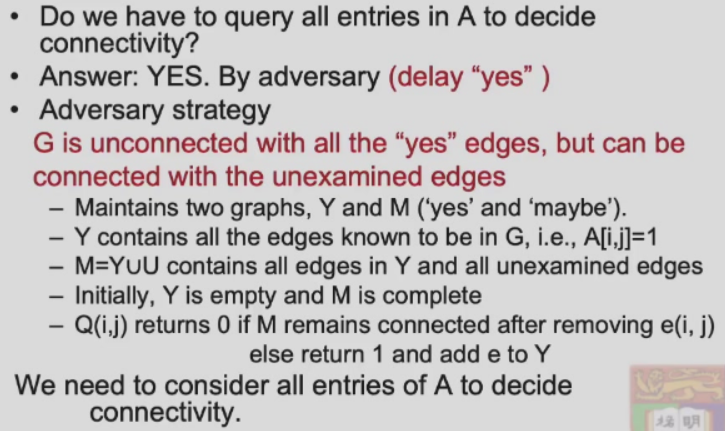
\includegraphics[width=0.309\textwidth]{pic/DAA5/Graph Connectivity}
        \caption{Graph Connectivity}
    \end{figure}
    
    \item Containment of 2 non-adjacent edges
    \begin{definition}
        A property is \textbf{critical} for a property if it gains that property by answering YES to any uncertain edge.
    \end{definition}
    \begin{figure}[H]
        \centering
        \begin{subfigure}{0.48\textwidth}
            \centering
            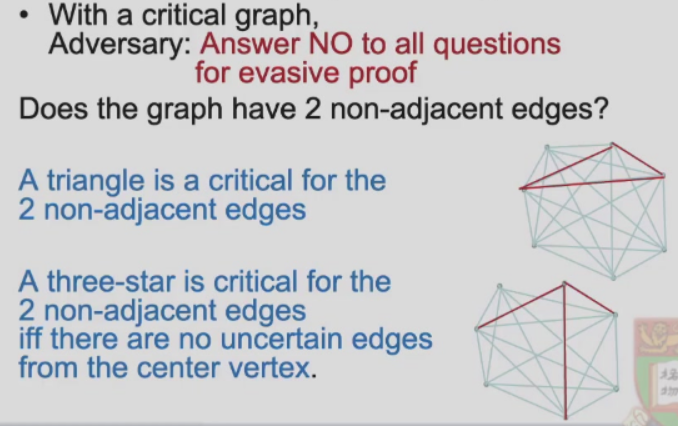
\includegraphics[width=0.618\textwidth]{pic/DAA5/Containment of 2 non-adjacent edges}
            % \caption{}
        \end{subfigure}
        \begin{subfigure}{0.48\textwidth}
            \centering
            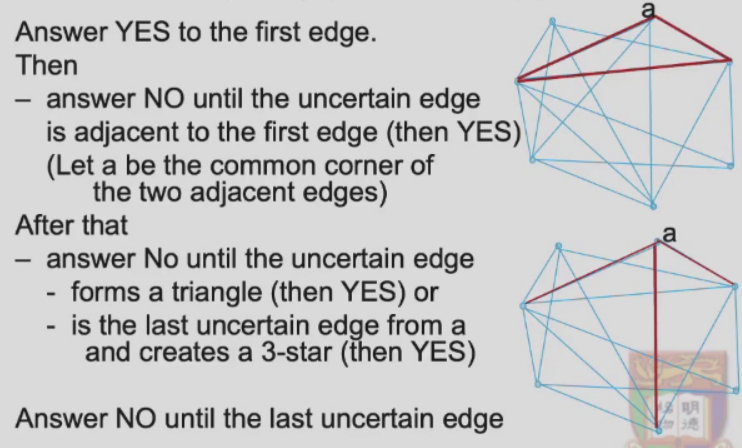
\includegraphics[width=0.618\textwidth]{pic/DAA5/Containment of 2 non-adjacent edges proof.png}
            % \caption{}
        \end{subfigure}
        \caption{Containment of 2 non-adjacent edges}
    \end{figure}
    
    \item 2-path(2 adjacent edges)
    \begin{figure}[H]
        \centering
        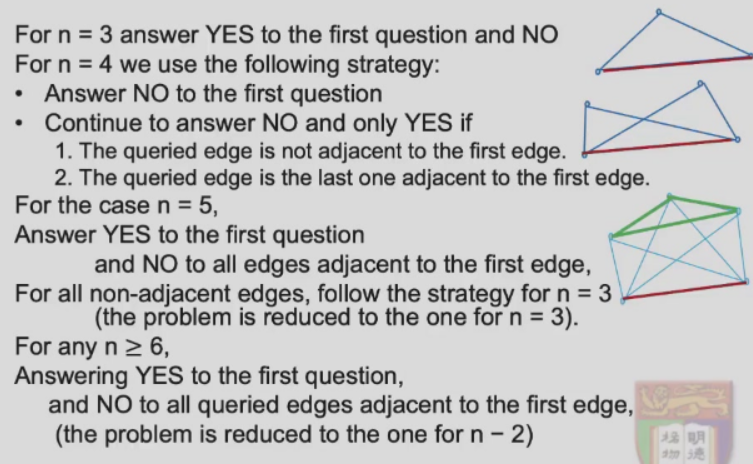
\includegraphics[width=0.309\textwidth]{pic/DAA5/2 adjacent edges}
        \caption{2 adjacent edges}
    \end{figure}
    \item Maximum Star
    \begin{figure}[H]
        \centering
        \begin{subfigure}{0.48\textwidth}
            \centering
            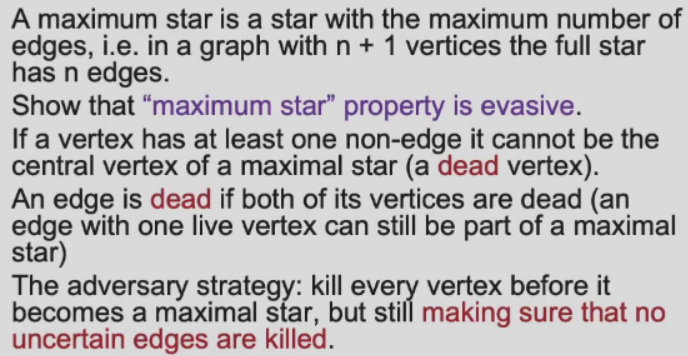
\includegraphics[width=0.618\textwidth]{pic/DAA5/Maximum Star1}
        \end{subfigure}
        \begin{subfigure}{0.48\textwidth}
            \centering
            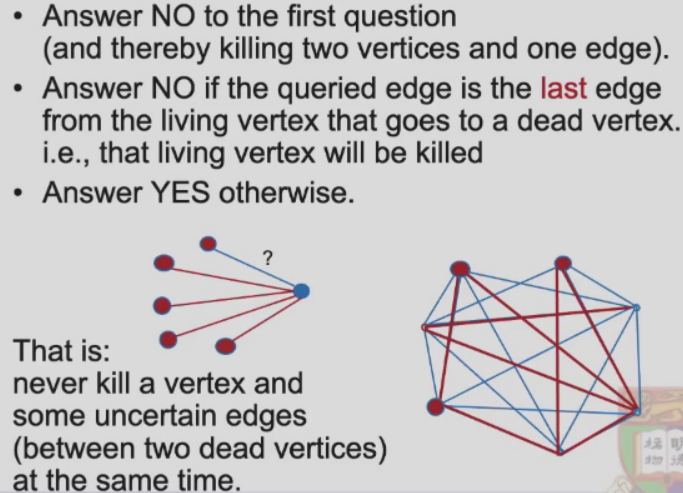
\includegraphics[width=0.618\textwidth]{pic/DAA5/Maximum Star2}
        \end{subfigure}
        \caption{Maximum Star}
    \end{figure}
\end{itemize}

\subsubsection{A Conjecture on Evasiveness}

\begin{figure}[H]
    \centering
    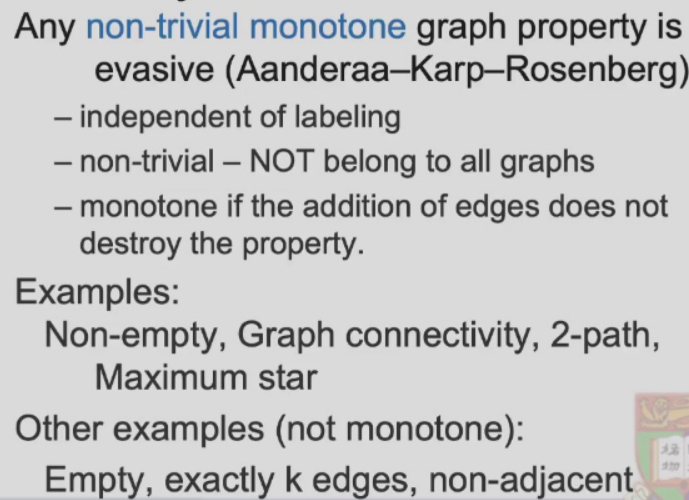
\includegraphics[width=0.309\textwidth]{pic/DAA5/A Conjecture on Evasivenes}
    \caption{A Conjecture on Evasivenes}
\end{figure}



\subsection{Non-evasiveness}
\subsubsection{Scorpion}
\begin{figure}[H]
    \centering
    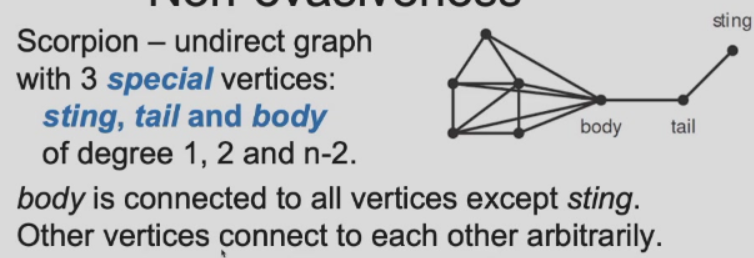
\includegraphics[width=0.309\textwidth]{pic/DAA5/Scorpion}
    \caption{Scorpion}
\end{figure}

Non-evasiveness with $<5n$ queries.

\begin{figure}[H]
    \centering
    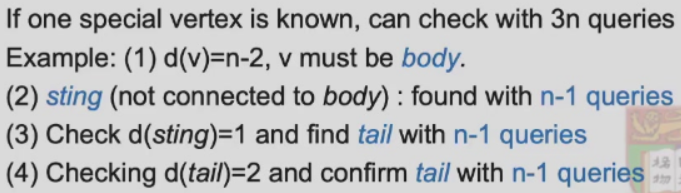
\includegraphics[width=0.309\textwidth]{pic/DAA5/Scorpion check}
    \caption{Scorpion check}
\end{figure}

\begin{figure}[H]
    \centering
    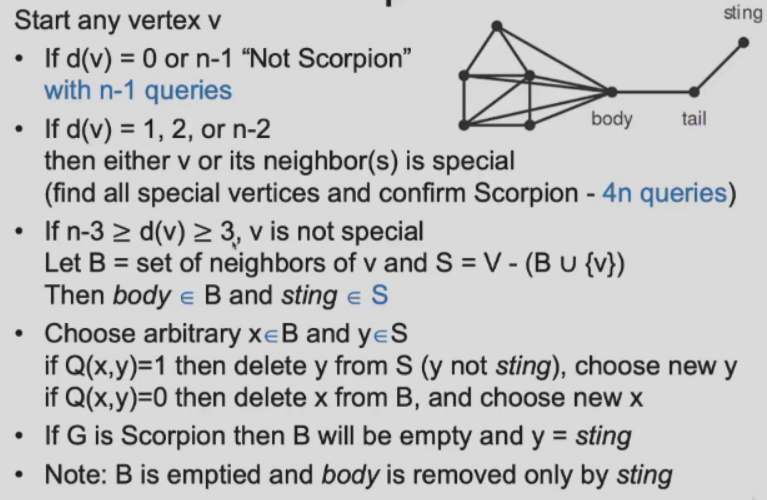
\includegraphics[width=0.309\textwidth]{pic/DAA5/Scorpion proof.png}
    \caption{Scorpion proof}
\end{figure}

\subsubsection{Sink}
\begin{figure}[H]
    \centering
    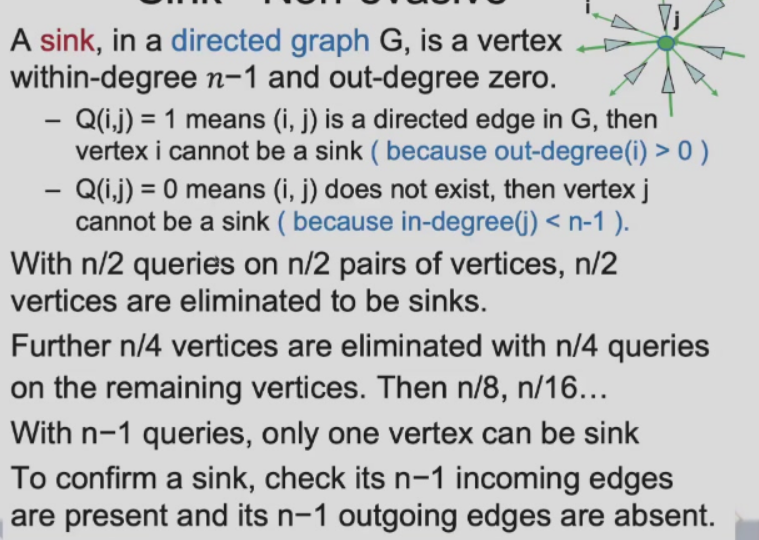
\includegraphics[width=0.309\textwidth]{pic/DAA5/Sink}
    \caption{Sink}
\end{figure}



\subsection{Evasive Property for String}
\begin{definition}
    A string property is \textbf{evasive} if any algorithm that determines that property must evaluate every input bit in worst case.
\end{definition}

\begin{figure}[H]
    \centering
    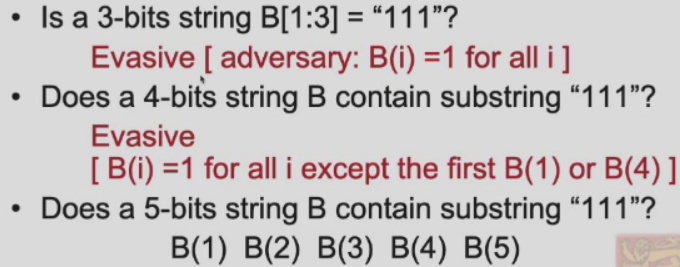
\includegraphics[width=0.309\textwidth]{pic/DAA5/Evasive Property for String exp}
    \caption{Evasive Property for String Example}
\end{figure}
5-bits is not evasive.

\subsubsection{Finding Patterns in Bit Strings}
Does a $n$-bits string $B$ contain the substring $01$?

\begin{figure}[H]
    \centering
    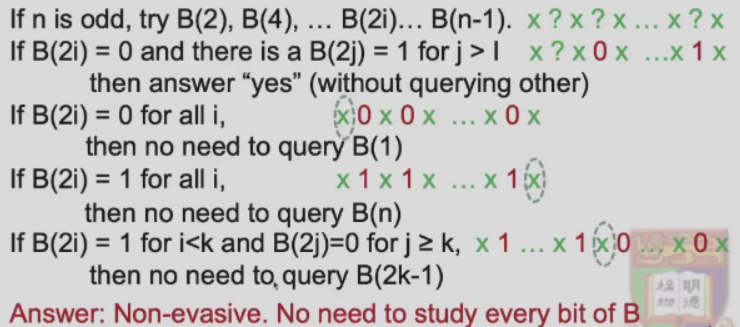
\includegraphics[width=0.309\textwidth]{pic/DAA5/Finding Patterns in Bit Strings}
    \caption{Finding $01$ Patterns in Odd-Length $B$}
\end{figure}


\begin{figure}[!htb]
    \centering
    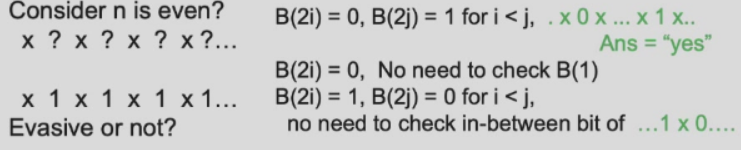
\includegraphics[width=0.309\textwidth]{pic/DAA5/Finding Patterns in Bit Strings2}
    \caption{Finding $01$ Patterns in Even-Length $B$}
\end{figure}


\begin{figure}[H]
    \centering
    \begin{subfigure}{0.48\textwidth}
        \centering
        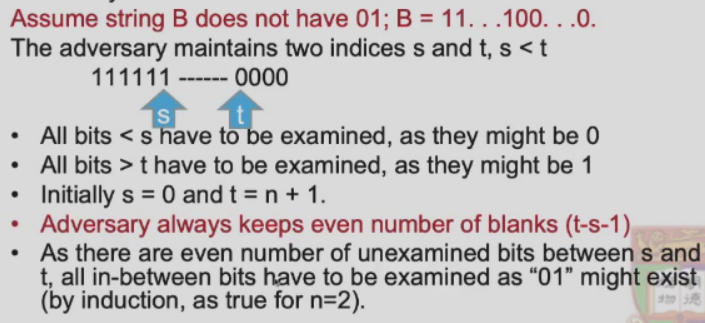
\includegraphics[width=0.618\textwidth]{pic/DAA5/Adversary1}
        % \caption{}
    \end{subfigure}
    \begin{subfigure}{0.48\textwidth}
        \centering
        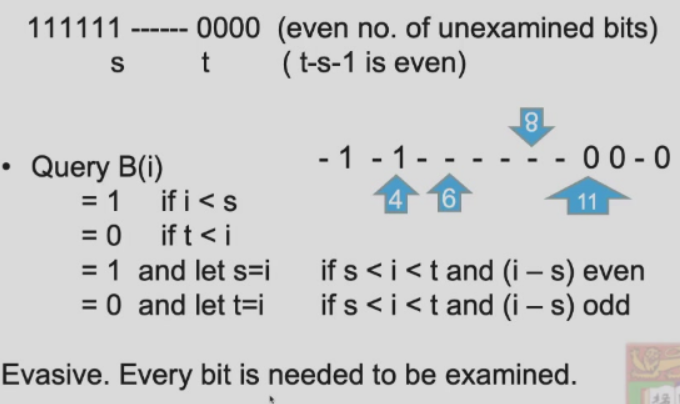
\includegraphics[width=0.618\textwidth]{pic/DAA5/Adversary2}
        % \caption{}
    \end{subfigure}
    \caption{Adversary}
\end{figure}

\subsubsection{Other String Problems}
\begin{figure}[H]
    \centering
    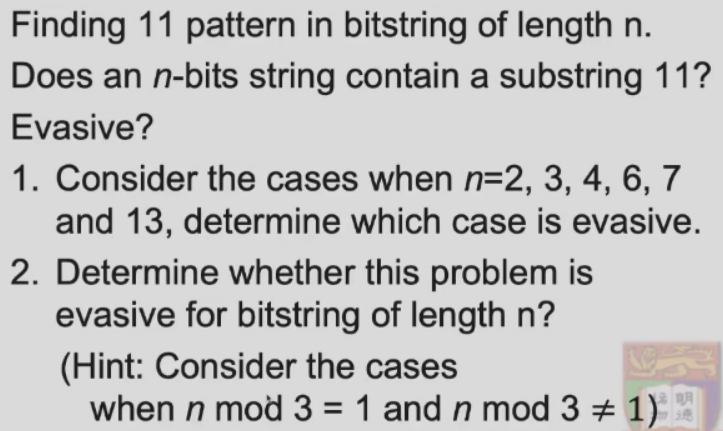
\includegraphics[width=0.309\textwidth]{pic/DAA5/Other String Problems}
    \caption{Other String Problems}
\end{figure}
